
\documentclass[fleqn,usenatbib]{mnras}


\usepackage{newtxtext,newtxmath}

% Use vector fonts, so it zooms properly in on-screen viewing software
% Don't change these lines unless you know what you are doing
\usepackage[T1]{fontenc}


\DeclareRobustCommand{\VAN}[3]{#2}
\let\VANthebibliography\thebibliography
\def\thebibliography{\DeclareRobustCommand{\VAN}[3]{##3}\VANthebibliography}


%%%%% AUTHORS - PLACE YOUR OWN PACKAGES HERE %%%%%

% Only include extra packages if you really need them. Common packages are:
\usepackage{graphicx}	% Including figure files
\usepackage{amsmath}	% Advanced maths commands

\title[Short title, max. 45 characters]{The Fate of our Sun Analogs in the Andromeda Galaxy, and Star Migration Within}


\author[Paarth Parab et al.]{
Paarth Parab
\\
}
% These dates will be filled out by the publisher
\date{May 5 , 2023}

% Don't change these lines
\begin{document}
\label{firstpage}
\pagerange{\pageref{firstpage}--\pageref{lastpage}}
\maketitle

% Abstract of the paper
\begin{abstract}
We look at how the Sun Analogs in the Andromeda Galaxy change over time during the merger process with the Milky Way, as well as the movement of solar particles within the galaxy. This important for learning about galaxy evolution and how the components of galaxies change during a merger, as well as the potential fate of our Sun and stars alike. This paper will be exploring the fate of Sun analogs within the Andromeda Galaxy, wondering what happens during the merger process. This question is important to learn what could happen to our own Sun and solar systems all around. The first finding was that a majority of our Sun analogs in M31 move radially outward over time, and even more so in the merger process, and some that actually gravitate towards the center of the galaxy strongly. The other important finding was what happens to the solar particles within this range of 7.4 - 8.7 kpc, which was that many more end up occupying this region by the end of the merger. The Sun analogs moving all over the place is showing the gravitational forces from the Milky Way and how the metallicity changes impact the regions of the merger remnant. Proving that the solar particles gravitate outwards naturally in the spiral arms, where more star development is found.
\end{abstract}

\begin{keywords}
Galaxy Merger, 
Galaxy Interaction,  
Merger Remnant, 
Elliptical Galaxy,
Spiral Galaxy
\end{keywords}

\section{Introduction}

\paragraph{}
When the merger of our galaxy with Andromeda takes place, the Sun analogs that reside in M31 are a mystery as to what happens. However, it is believed that those Solar Particles will actually move radially outwards of the Merger Remnant. A Merger Remnant is the final product of multiple galaxies colliding, and combining to form one galaxy. In this paper I am going to go over the fate of the stars in M31, that are the same distance from the center of the galaxy like our sun is, about 8 kpc away from the center of the galaxy. This is for the galaxy merger process and after the merger completes. A galaxy merger is when multiple galaxies collide, and the gravitational pull forces the galaxies to become one. 

\paragraph{}
Knowing what happens to these stars in the galaxy and running simulations will tell us more about what could possibly happen to our solar system and the Milky Way in the future, and just the general structure as well for M31 at this distance within. 
"A galaxy is a gravitationally bound collection of stars whose
properties cannot be explained by a combination of baryons and
Newton’s laws of gravity."
This is the definition of a galaxy from (Willman \& Strader 2012 AJ). 
Galaxy evolution however is the galaxy changing its components over time as stars get more massive, gas forms new stars, and even the colors can change. 
From running simulations, we can also find out what happens to the stars physically and chemically at this distance, and see how it impacts that region for the dust and gas. We can also find out the change of velocities, and then find the new distance these stars will be at after the merger.

\paragraph{}
We know that by the time the collision begins, our Sun will be a red giant and will have already ate up Mercury, Venus, and maybe Earth. We also know that when the merger takes place the final product galaxy will end as a giant elliptical galaxy, changing the structure for the spiral arms and the dust and gas ratios within the distance. 
An elliptical galaxy is a galaxy that is in an ellipsoid shape with long arms. The Sun will most likely end up at a larger distance from the center of the Milky Way and Andromeda merged galaxy, than it is currently from the center of the Milky Way. Possibly more than 50 kpc.
(van der Marel + Besla, 2012).
Figure 1 is that of the radial distribution of the candidate suns with respect to the MW and M31 remnant. 
Knowing that the galaxies are fairly similar in many characteristics, we can use our own estimation of the Sun to help find what could happen to the M31 stars. 

\paragraph{}
Active questions in the field include:
\begin{itemize}
  \item How will the local density of stars change? 
  \item How could the stars pass by the systems and potentially change the system structure as well as the stars compositions?
  \item If Earth is still around, how could life be impacted?
  \item How do the positions of the Sun analogs change? (In merged remnant vs. today)
\end{itemize}

\paragraph{}
The star counts were looked at for M31 and projections have been made about the Luminosity and Intensity profiles. Mainly looking at the semimajor and semiminor axes of the disk. (Courteau + Widrow IOP, 2011)
\begin{figure}
\graphicspath{ {/home/} }
\includegraphics[width=7cm, height=5cm]{research2image}
\caption{This image is a graph of the fraction of Sun Analogs of M31 over the distance from the Merger Remnant. This is from after the simulation has finished, and shows that a higher fraction of Sun Analogs are actually going to be moving away from center of the Remnant. It is believed then that our Sun will actually move outwards radially as well. (van der Marel + Besla, 2012)
}
\end{figure}



\section{This project}

In this paper we will study the Sun analogs in M31. We will look at the original positions of these analogs in the xy-plane, then showing how it changes over time and as the merger takes place, through a face on view. We will look at the movement of these analogs over time, and see what has changed. Another important thing we will be looking at will be how the amount of Solar particles within 7.4 - 8.7 kpc change over time and the merger process.
\paragraph{}
The main question to answer is, how do the positions of the Sun analogs change as the merger takes place and where do they end up in the Merger Remnant?
\paragraph{}
This is important to know for how the stars move around in a galaxy when the mergers take place, thinking about the gravitational components of the new Merger Remnant, and how the two spiral galaxies will create one big elliptical galaxy. A spiral galaxy is a galaxy that is a flat rotating disk, with a central concentration of stars near the center known as a "Bulge". This is also important so we know the behavior of certain stars and how they flow within the merger process. The study in this paper will help us better understand how these Sun analogs behave during the merger process and how they will impact the new formation of the Merger Remnant. 


\section{Methodology}

The simulations I will be using are for the MW and M31 merger and studying the stars that are about 7.4 - 8.7 kpc away from center of the galaxy. An N-body simulation is where there are an N number of particles and simulates the movement of the particles, randomly but with respect to gravity and physical equations. (van der Marel + Besla, 2012)

\paragraph{}
To find the positions of the Sun analogs, I will use the data for the stars that are within 7.4 - 8.7 kpc of the center in M31 and track those solar particles over time. I am using 7.4 - 8.7 kpc as the distance because our Sun is about 8.29 kpc away, but it still fluctuates. Then seeing how many stars are within this distance before the merger begins, and seeing how many are there after the merger finishes. Also seeing how the star density changes at the different regions around the center, and going outward to see how the other regions changed as well. 
Looking at Figure 2, I will focus on how these solar particles change for M31 and how the density of these solar particles in the regions changes over time.


\begin{figure}
\graphicspath{ {/home/} }
\includegraphics[width=7cm, height=4cm]{image2research2}
\caption{This image is of the Solar particles tracked for MW and M31 at the end of the merger. Respectively, there is still some settling for the solar particles but the density of solar particles is heavy and luminous. (van der Marel + Besla, 2012)
}

\end{figure}

\paragraph{}

My code will compute how much of the Sun analogs stayed in the same positions and how many of them moved. Seeing the amount that are there at the start of the simulation and then the amount that are there at the end. Also during the intervals, keeping a running count of the snapshots and time. Mainly making a visual movie of how the M31 solar particles change over time, and another plot to show how many solar particles are within the Sun Analog range, over the whole process.

\paragraph{}
The plots I need to make are the xy-plane of the two galaxies during the merger process. A face-on view will give a clear view of where the Sun analogs are then over a movie type simulation, show the movement of the stars. Also making a plot of how many solar particles are within the Sun Analog range to show just exactly how the stars move around and where they gravitate towards. 

\paragraph{}
I believe that within 8.5 kpc of the center of the galaxy for M31, the amount of stars will be less. More specifically I believe that many other stars will occupy this space, and many stars from before will be much farther. So less stars than before the merger, but many new stars in this region that came from further. The fate of the stars in this region to me is very random, many stars being pushed further, and some going through collisions and potential chemical changes. I believe this happens from the new gravitational components of the Elliptical Merger Remnant, as well as the general structure of the MW - M31 remnant changing and settling in to a new structure.

\section{Results}

The first set of figures is the face-on visuals for the solar particles that are within 7.4 - 8.7 kpc from the center of M31. The first image (Figure 3) is that of the current day, then the second image (Figure 4) is that of those same solar particles but during the merger process about 8.5 Gyr in the future. The third image is that of the final product of the merged galaxies, the Merger Remnant of Andromeda and the Milky Way. As we can see those Sun Analogs are all over the place, many which have gravitated outwards and many of which have also gone near the center of the Merger Remnant.

\begin{figure}
\graphicspath{ {/home/} }
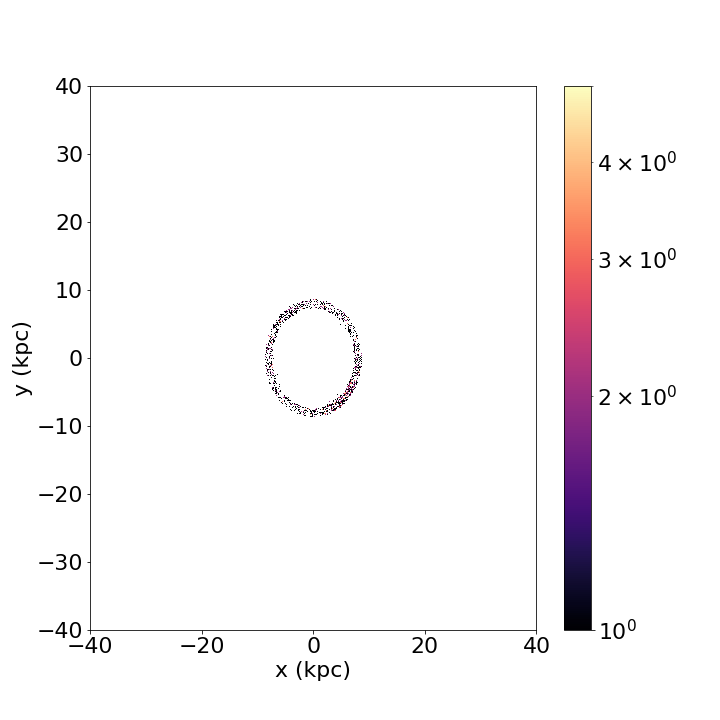
\includegraphics[width=7cm, height=7cm]{FaceOn_Density000}
\caption{This figure is that of M31's Sun analogs at the current moment in time. Everything in the image looks nice and neat, the solar particles just fluctuating within this region itself.
}

\end{figure}

\begin{figure}
\graphicspath{ {/home/} }
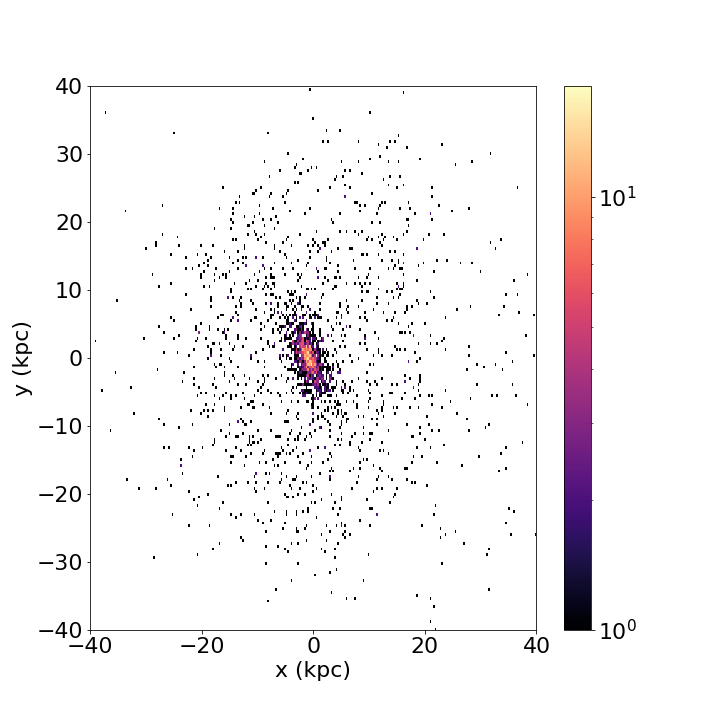
\includegraphics[width=7cm, height=7cm]{FaceOn_Density350}
\caption{This figure is that of those M31's Sun analogs in the middle of the merger process, about 5 Gyr in the future. Now this is where things get crazy, many of those particles have moved outward, and the higher density we see near the center is actually the solar particles that moved inward more due to the gravity and collisions of the Milky Way coming in.
}

\end{figure}

\begin{figure}
\graphicspath{ {/home/} }
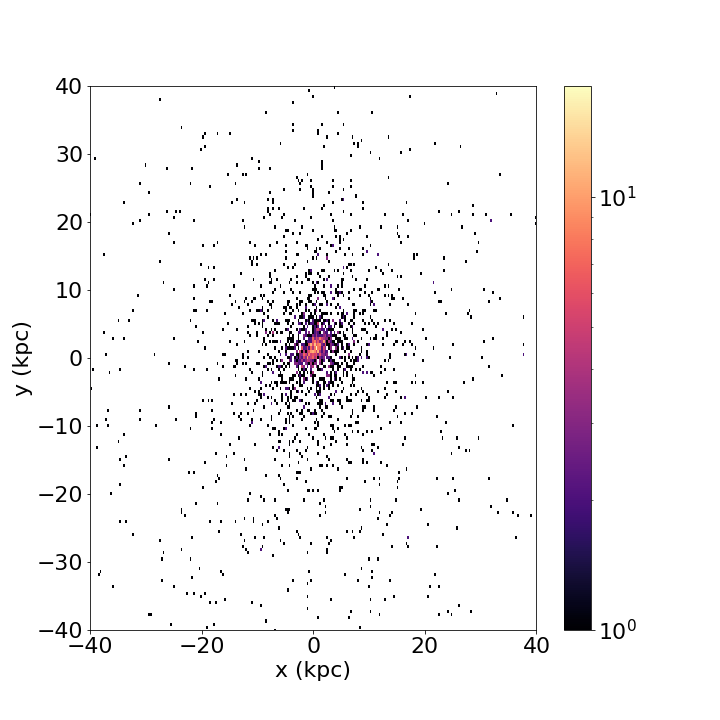
\includegraphics[width=7cm, height=7cm]{FaceOn_Density800}
\caption{This figure is that of those M31's Sun analogs at the end of the merger process, for the Merger Remnant, about 11.4 Gyr in the future. As we can see there is still a lot of settling to do for the solar particles, many of which we can see have moved way far out, and have gone all over the place. Showing how when the merger takes place, for those Sun analogs, a majority have moved outward and maybe even some become unbound.
}

\end{figure}


\paragraph{}
The next steps to better understand what happens within M31 during this whole process, was to look at the Sun analog range and see how many solar particles are occupying this region as time goes on. Many particles are actually moving into this region, and that is believed to be because of the gravitational components moving these stars around all over the place within the galaxy. The major dip that happens around 5.5 - 6 Gyr from now is due to the extreme moving around of the solar particles during the merger from inflow of gas and gravity. Many of which are being gravitationally disrupted and moving to all kinds of places within the galaxy. Then as time goes on the solar particles once again settle in certain regions.

\begin{figure}
\graphicspath{ {/home/} }
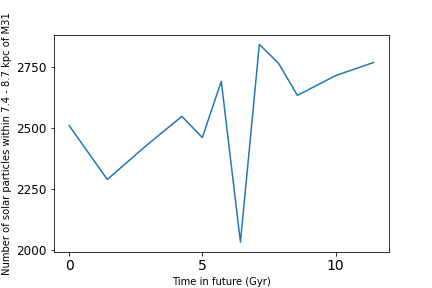
\includegraphics[width=9cm, height=7cm]{graphofsolarparticles}
\caption{This is a graph of the amount of solar particles that are within the Sun analog range over time. Seeing clearly how it jumps all over the place, we see that during the merger process later on, the amount of solar particles within this region are actually increasing. Showing how the new gravitational component from the Milky Way is impacting this region significantly.
}

\end{figure}


\section{Discussion}

This result does somewhat agree with my hypothesis. We know that because we have a spiral galaxy, the stars will gravitate more outwards as time goes on due to stars forming in the spiral arms. This is due to the anatomy of spiral structures, which are the reason for the heavy star migration within a galaxy. (Rok and Debattista, 2012). So as time goes on during the merger process, the stars will actually be moving all over the place, so for the merger remnant it makes sense that the stars will be at a much larger distance from the center of the galaxy. This makes sense as for the Sun analogs, it was found in another paper that about 85 percent of those Sun analogs will be at a distance greater than where they started. (van der Marel + Besla, 2012). This is important for many reasons such as the migration of stars, and is important how it can correlate to the new elliptical galaxy of the merger remnant. The metallicity in the merging galaxies is actually changing significantly however. This also is a huge reason for the way stars are being pushed around within the merger process, as seen in Figure 6, another reason for the huge dip and stars moving all over the place. This is due to the metallicity dilution and chemical enrichment. (Torrey and Cox, 2012). This is a natural reaction to the merger process, as well as the major gas inflow to help with more nuclear star formation of the new Merger Remnant. 

\paragraph{}

Uncertainties include not looking at every snapshot of data, instead of iterating over all 800 snapshots of data I instead used every 50 snapshots for 16 snapshots to use. Using the whole 800 would take a long time and maybe certain points in those data sets might have been a little off. Other uncertainties include the data set itself, this data set could be a bit different than the data sets used in other research and papers. Other uncertainties could be from the amount of screenshots especially for the graph, which could be more accurate using all snapshots.


\section{Conclusion}

When our Milky Way galaxy merges with the Andromeda galaxy, many changes happen within the galaxies and solar particles move all over the place. Over time, our Sun analogs in the Andromeda galaxy move all over the place, a majority of which move radially outwards. Over time and the merger process, the Galaxy Interaction, the galaxies are spiralling and moving solar particles all over the place causing massive gravitational disruption within the galaxies. A Galaxy Interaction is when multiple galaxies interact, doesn't have to be during the merger process, but can start when the gravity forces begin to change the components within each galaxy involved, like we see strongly with Andromeda and our Milky Way. Also showing how the metallicity and chemical enrichment impact the solar particles movement. 

\paragraph{}

The most important findings were about how impactful the gravitational components are during the merger process itself. How the metallicity changing impacts the gas flow causes the solar particles to really get pushed around. Including how over time within M31 the stars naturally go outward, due to being a spiral galaxy, and also the gravitational impact from the Milky Way getting closer and closer. The dip in the Figure 6 occurs from the Milky Way and Andromeda beginning the collision and in the middle of settling. Then those solar particles in M31 begin to occupy that region and even more so in the center, as the Milky Way solar particles come in to occupy more regions near the outside of the Merger Remnant as well. 

\paragraph{}

I believe the future of this topic is going to be interesting the more time goes on. We will see more data come in and get a better understanding of how exactly things will change not just for our galaxies but what could potentially happen to our solar system and life on Earth, if it were still around. A possibility for life elsewhere could happen as well potentially during the merger process or in the final Merger Remnant. To explore more into this topic, one could compare other galaxy mergers and as well as bringing in the full impact of M33 which will also join in this merger later on in time. Another huge thing would be to deeply look at how the metallicity changes before the merger gets close and how the gas flow is being impacted at that time as well, then how the gas and dust change after the merger has completed. My code wasn't getting the best of the data, if I had used more screenshots and at a better rate maybe focusing on the merger itself, more things could have been found. I do believe that this code gives a great visual as to how impactful this merger is for our galaxies and merger of galaxies all over. The fate of our Sun analogs, should no longer be a mystery. 

\section{Acknowledgements}

1. Astropy (Astropy Collaboration et al. 2013; Price-Whelan et al. 2018 doi: 10.3847/1538-
3881/aabc4f)
\\
2. matplotlib Hunter (2007),DOI: 10.1109/MCSE.2007.55
\\
3. numpy van der Walt et al. (2011), DOI : 10.1109/MCSE.2011.37
\\
4. scipy Jones et al. (2001–),Open source scientific tools for Python. http://www.scipy.org/
\\
5. Dr. Gurtina Besla, help of code from class







%%%%%%%%%%%%%%%%%%%% REFERENCES %%%%%%%%%%%%%%%%%%

% The best way to enter references is to use BibTeX:

\nocite{*}
\bibliographystyle{plain}
\bibliography{citations.bib}




% Alternatively you could enter them by hand, like this:
% This method is tedious and prone to error if you have lots of references
%\begin{thebibliography}{99}
%\bibitem[\protect\citeauthoryear{Author}{2012}]{Author2012}
%Author A.~N., 2013, Journal of Improbable Astronomy, 1, 1
%\bibitem[\protect\citeauthoryear{Others}{2013}]{Others2013}
%Others S., 2012, Journal of Interesting Stuff, 17, 198
%\end{thebibliography}

%%%%%%%%%%%%%%%%%%%%%%%%%%%%%%%%%%%%%%%%%%%%%%%%%%

%%%%%%%%%%%%%%%%% APPENDICES %%%%%%%%%%%%%%%%%%%%%

\appendix


%%%%%%%%%%%%%%%%


% Don't change these lines
\bsp	% typesetting comment
\label{lastpage}
\end{document}

% End of mnras_template.tex
